% Search for all the places that say "PUT SOMETHING HERE".

\documentclass[11pt]{article}
\usepackage{amsmath,textcomp,amssymb,geometry,graphicx}

\def\Name{Jianzhong Chen}  % Your name
\def\Login{ee122-bv} % Your login
\def\Homework{3}%Number of Homework, PUT SOMETHING HERE
\def\Session{Fall 2013}


\title{EE122--Fall 2013 --- Solutions to Homework \Homework}
\author{\Name, \texttt{\Login}}
\pagestyle{myheadings}

\begin{document}
\maketitle

\section*{Problem 1}
a)\\
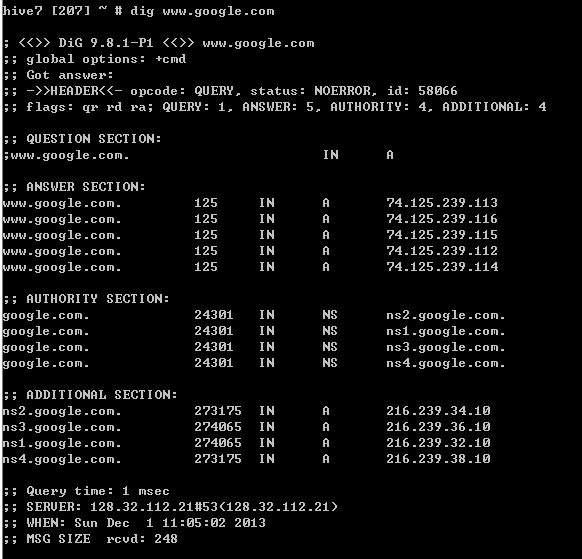
\includegraphics[scale=0.5]{122-hw3-1}\\
Name=www.google.com\\
TTL=125\\
Class=IN\\
Type=A\\
Value=74.125.239.113\\
\newpage
b)\\
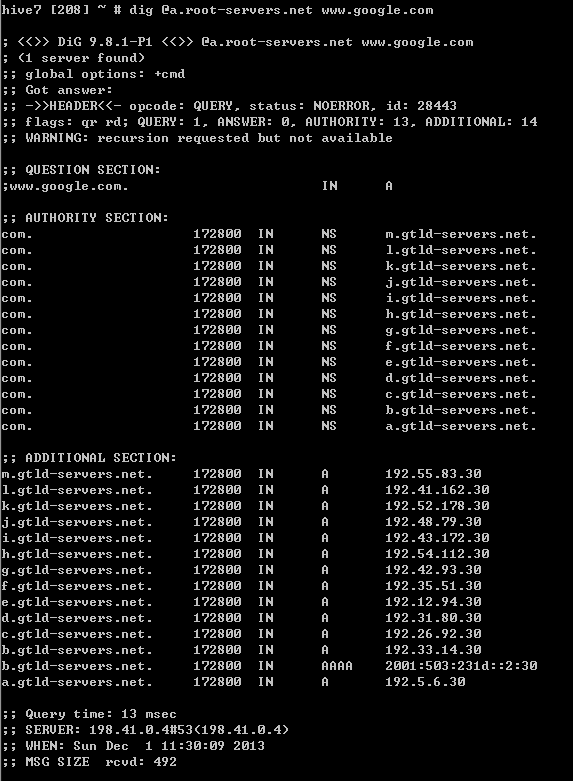
\includegraphics[scale=0.38]{122-hw3-2}\\
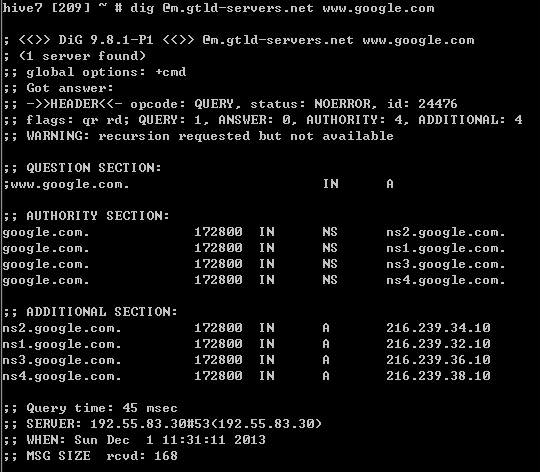
\includegraphics[scale=0.38]{122-hw3-3}\\
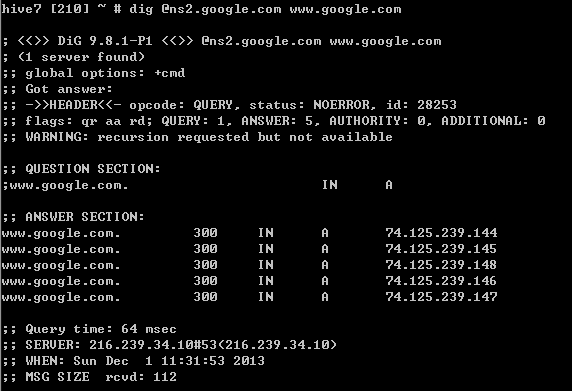
\includegraphics[scale=0.38]{122-hw3-4}\\
a.root-servers.net$\rightarrow$n.gtld-servers.net$\rightarrow$ns2.google.com\\
a.root-servers.net is responsible for *\\
n.gtld-servers.net is responsible for *.com\\
ns2.google.com is responsible for *.google.com\\
\newpage
c)\\
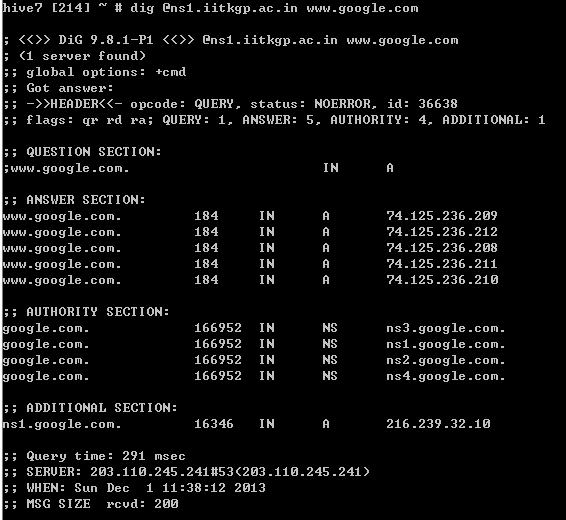
\includegraphics[scale=0.5]{122-hw3-5}\\
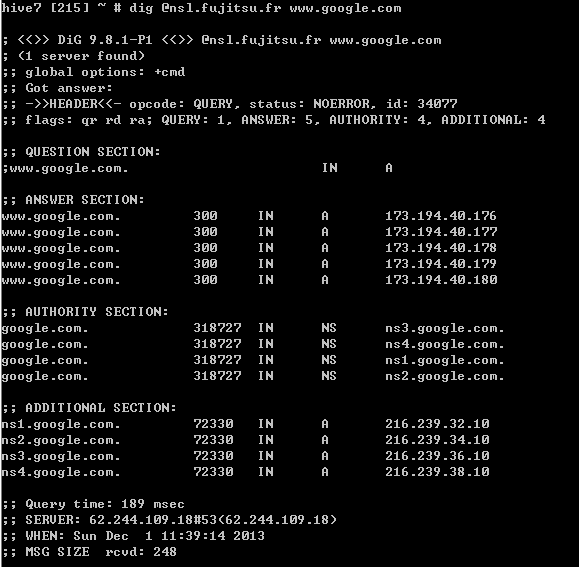
\includegraphics[scale=0.5]{122-hw3-6}\\
The latency that was returned by my default DNS server is much less than that returned by these two servers. Because the google server for the ip address returned by our default DNS server is much closer to us.
\newpage
d)\\
dig www.google.com\\
\\
Answers:\\
(no response)\\
Authority section:\\
ns1.google.com 3600 IN NS ns.evilsearch.com\\
Addition:
ns.evilsearch.com IN A xxx.xxx.xxx.xxx\\
\\
check whether the returned domain server name is a legal, or 'evil free' using a provided list such as the computer user's organization or an Internet service provider (ISP)
\label{pg:end-of-p1}


%Insert solution here


% Make sure that the solution here does not exceed one page here. If
% it does, use the extra space for this problem at the end.  
%
% Comment out the next line if you are NOT using the extra space
%\paragraph{} \emph{Continued on Page \pageref{pg:p1-continuation}}
\newpage


%%Do NOT remove/comment the next line
\pagestyle{plain}
%%It makes sure your name appears only on the first page
\section*{Problem 2}
\begin{enumerate}
\item R+R+4*(R+R)=10R
\item R+R+4R=6R
\item R+R+R+R=4R
\item R+R+4*($\dfrac{1}{2}$R+$\dfrac{1}{2}$R)=6R
\item R+R+$\dfrac{1}{2}$R+4*$\dfrac{1}{2}$R=4.5R
\item R+R+$\dfrac{1}{2}$R+$\dfrac{1}{2}$R=3R
\item R+R+2*($\dfrac{3}{4}$R+$\dfrac{1}{2}$R+$\dfrac{1}{3}$R+$\dfrac{1}{4}$R)=$\dfrac{17}{3}$R
\item R+R+2*($\dfrac{3}{4}$R+$\dfrac{1}{2}$R+$\dfrac{1}{3}$R+$\dfrac{1}{4}$R)=$\dfrac{17}{3}$R
\item R+R+2*$\dfrac{3}{4}$R=3.5R
\end{enumerate}
\label{pg:end-of-p2}

%Insert solution here

% Make sure that the solution here does not exceed one page here. If
% it does, use the extra space for this problem at the end.  
%
% Comment out the next line if you are NOT using the extra space
%\paragraph{} \emph{Continued on Page \pageref{pg:p2-continuation}}
\newpage

\section*{Problem 3}
\begin{enumerate}
\item E$\rightarrow$B
\begin{enumerate}
\item CS
\begin{enumerate}
\item X=A,Y=B: Yes;No, because B is listening E's transmission, A's data blend with E's data and result in noise; Yes, because there is a noise occur.
\item X=F,Y=C: Yes;Yes;No Because in this case E and F are speaking, B and C are listening, no node is affected.
\item X=C.Y=A: Yes;Yes, because A is not listening to anyone when C decides to send data to A; Yes, because the broadcast of C blend with E's, and result in noise.
\end{enumerate}
\item MACA
\begin{enumerate}
\item X=A,Y=B: No, because A received CTS from B.
\item X=F,Y=C: No, because B's CTS blend with F's RTS and results in noise.
\item X=C.Y=A: No, because C received CTS from B.
\end{enumerate}
\end{enumerate}
\item B$\rightarrow$E
\begin{enumerate}
\item CS
\begin{enumerate}
\item X=A,Y=B: No, because B is speaking.
\item X=F,Y=C: Yes;No, because F's data blend with B's data; No, the origin transmission would not be affected.
\item X=C.Y=A: No, because C's data blend with B's data and results in noise to A.
\end{enumerate}
\item MACA
\begin{enumerate}
\item X=A,Y=B: No, because B could not response to A's RTS with CTS when transmitting data to E.
\item X=F,Y=C: No, because F's CTS blends with B's data and results in noise to B.
\item X=C.Y=A: No, because B's data broadcasting will results in noise to A and C.
\end{enumerate}
\end{enumerate}
\item A$\rightarrow$B
\begin{enumerate}
\item CS:None
\item MACA:None
\end{enumerate}
\item
\begin{enumerate}
\item CS:Yes, because D,E,F are speaking and A,B,C are listening, there is no collision.
\item MACA:Yes, because D,E,F send RTS to A,B,C; A,B,C send CTS to neighbors; before A,B,C receive CTS from each other, their own CTS were sent out to D,E,F; then D,E,F start to transmitting data with no collision.
\end{enumerate}
\item
Ideal: All of these, because for an ideal scenario, all nodes can simultaneously speak and listen.\\
CS: None of these, because for a node using CS, it can either speak or listen, but not both.
MACA: All of these, for D$\rightarrow$A, E$\rightarrow$B, F$\rightarrow$C, it is the same scenario with question 4. And for A$\rightarrow$D, B$\rightarrow$E, C$\rightarrow$F, A,B,C only receive RTS but no CTS from nodes other than D,E,F correspondingly for pairs (D,A)(E,B)(F,C), so the data can be transmitted without collision.
\end{enumerate}
\label{pg:end-of-p3}

% Make sure that the solution here does not exceed one page here. If
% it does, use the extra space for this problem at the end.  
%
% Comment out the next line if you are NOT using the extra space
%\paragraph{} \emph{Continued on Page \pageref{pg:p3-continuation}}
\newpage

\section*{Problem 4}
\begin{enumerate}
\item
\begin{enumerate}
\item 4-1-0-2-3-5 with 0 is the root
\item 5-4-1-2-3 with 1 is the root
\end{enumerate}
\item transmission: switches $|$ end-hosts\\
b to c: 0,1,2,3,4,5 $|$ a,b,c,d,e,f,g\\
c to b: 2,0,1 $|$ b\\
d to c: 3,5,2 $|$ c,f\\
a to b: 0,1 $|$ b\\
a to g: 0,1,2,3,4,5 $|$ a,b,c,d,e,f,g
\item
b to c: floods\\
a to b: unicasts\\
c to b: floods\\
b to c: unicasts\\
a to b: unicasts\\
c to b: floods\\
b to c: unicasts\\
a to b: unicasts\\
c to b: floods\\
b to c: unicasts\\
a to b: unicasts\\
c to b: floods
\begin{enumerate}
\item
(transmission) fraction flooded $|$ fraction unicasted\\ 
(a to b): $\dfrac{0}{4}$ $|$ $\dfrac{4}{4}$\\
(b to c): $\dfrac{1}{4}$ $|$ $\dfrac{3}{4}$\\
(c to b): $\dfrac{4}{4}$ $|$ $\dfrac{0}{4}$
\item swap 2,3 and swap 11,12
\end{enumerate}
\end{enumerate}
\label{pg:end-of-p4}
\end{document}